\section{Evaluation}\label{sec:evaluation}

\textit{Wie wird gemessen, welche Ergebnisse waren zu erwarten, was wurde erreicht. Warum gibt es Abweichungen, welche Probleme enthält die Messmethode.\todo{raus}}

Im folgenden Abschnitt wird die implementierte Lösung hinsichtlich der Leistungs- und Qualitätsanforderungen (vgl. Abschnitt \ref{sec:requirements}) evaluiert. Da zum Zeitpunkt der Fertigstellung der Arbeit noch kein ausreichend umfangreicher realer Datensatz zur Verfügung stand, wurde der frei verfügbare MovieLens 1M \citep{movielens1m} Datensatz genutzt. Dieser besteht aus ca. 1 Million Nutzerbewertungen von 3.900 Nutzern für 6040 Kinofilme. Er wurde gewählt, da er bereits in zahlreichen Publikationen zur Ergebnisevaluation genutzt wird (u.a in \citep{Cacheda2011} und \citep{Herlocker:2002:EAD:593967.594047}) und so eine gute Vergleichbarkeit bei den Ergebnissen erzielt werden kann. Der Solr-Index wurde auf Basis der korrespondierenden Filmdaten aus offenen Datenquellen\footnote{http://www.themoviedb.org/, http://mymovieapi.com/} gefüllt, so dass pro Film zwanzig verschiedene Textfelder u.a. mit Titel, Beschreibungen, Schauspielernamen und Stichworten zum Film gefüllt waren.

\subsection{Ergebnisse}

\subsubsection{Leistung}

Zur Bestimmung der Leistung wurden jeweils die in Abschnitt \ref{sec:requirements} beschriebenen Anforderungen an die Anfragen pro Sekunde für die einzelnen Dienste geprüft. Als Referenzsystem wurde ein mit Ubuntu Server 12.04 betriebener Server genutzt der mit 16 GB RAM und einem Dual-Core Intel Xeon E31275 arbeiten konnte. Als Webserver bzw. Servlet-Container wurde Jetty\footnote{http://www.eclipse.org/jetty/} Version 8.1.12 hinter einem Nginx \gls{Reverse Proxy} genutzt.

Der Testplan wurde Apache Jmeter\footnote{http://jmeter.apache.org/} aufgebaut und durchgeführt. Er wird in einem eigenen Repository zur besseren Nachvollziehbarkeit zur Verfügung gestellt. \todo{Repo-Link}. Die einzelnen Messungen liefen, wenn nicht anders angegeben, jeweils 120 Sekunden mit einer vorgelagerten 30-sekündigen Ruhephase. Um den Einfluss von Netzwerklatenzen zu vermindern, wurde  alle Systeme in gleichen Rechenzentrum, d.h. innerhalb der selben Netzwerkstruktur, genutzt.

Die vollständige Auflistung der Messergebnisse für die einzelnen Systembestandteile und Konfigurationen befindet sich in Anhang \ref{app:performance}.

%\todo{raus}\begin{itemize} 
%\item Performance Tracker (req/s) - (concurrent con)
%\item Performance Solr Personalisierung 1 single core (req/s) - (concurrent con)
%\item Performance Solr Personalisierung 1 multi core / single recommender (req/s) - (concurrent con)
%\item Performance Solr Personalisierung 1 multi core / multi recommender (req/s) - (concurrent con)
%\item Performance Solr Personalisierung 2 single core (req/s) - (concurrent con)
%\item Performance Solr Personalisierung 2 multi core (req/s) - (concurrent con)
%\end{itemize}
\newpage

\paragraph{Tracker} Da die große Anzahl der zu erwartenden Anfragen auch eine sehr großen Zahl gleichzeitiger Verbindungen erfordert, wurden neben dem möglichen Durchsatz auch die maximal möglichen parallelen Verbindungen ermittelt. Um der normalen Nutzung des Dienstes zu entsprechen, wurde zufällige Trackingevents über die HTTP-Schnittstelle an den Dienst gesendet und die entsprechende Antwort geprüft.

Die Erwartung, dass der Dienst ab einer bestimmten Anzahl paralleler Anfragen neue Verbindungen nichtmehr annehmen kann und diese abweisen muss, wurde erfüllt. Wie in Abbildung \ref{fig:chart_tracker} deutlich wird, ist diese Schwelle bei ca. 350 gleichzeitigen Verbindungen erreicht. Dies hat zur Folge, dass der erziele Durchsatz stark einbricht und dass es zudem ab der Schwelle von ca. 600 parallelen Anfragen zudem zu Verbindungsabbrüchen kommt. Dies zeigt sich in der ebenfalls abgebildeten Fehlerquote.

Die Anforderungen an den maximalen Durchsatz erreicht bzw. übertrifft der so betriebene Dienst. Die Fehlerrate von 0\% wurde zudem bei dauerhaften Belastungen von 50 und 100 Anfragen pro Sekunden über einen Zeitraum von 30 Minuten bestätigt. 

\begin{figure}[H]
  \centering
    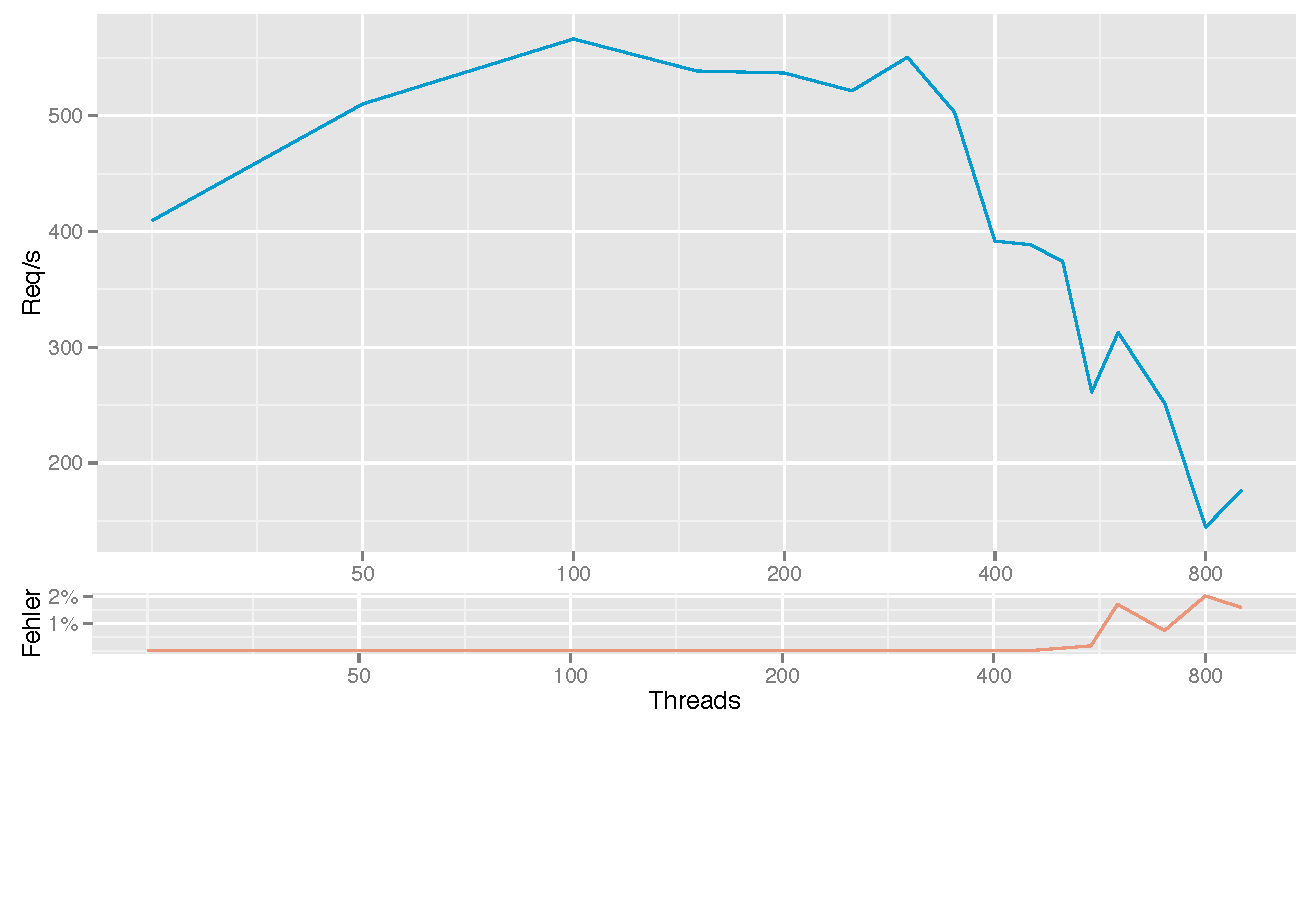
\includegraphics[width=\textwidth]{Abbildungen/tracker.pdf}
    \caption[Leistung Tracker]{Trackerleistungsdiagramm - Gegenüberstellung der Anzahl der parallel genutzten Threads, der erzielten Leistung und der Fehlerquote}
    \label{fig:chart_tracker}
\end{figure}

\paragraph{Personalisierung mit Webservice}

\begin{figure}[H]
  \centering
    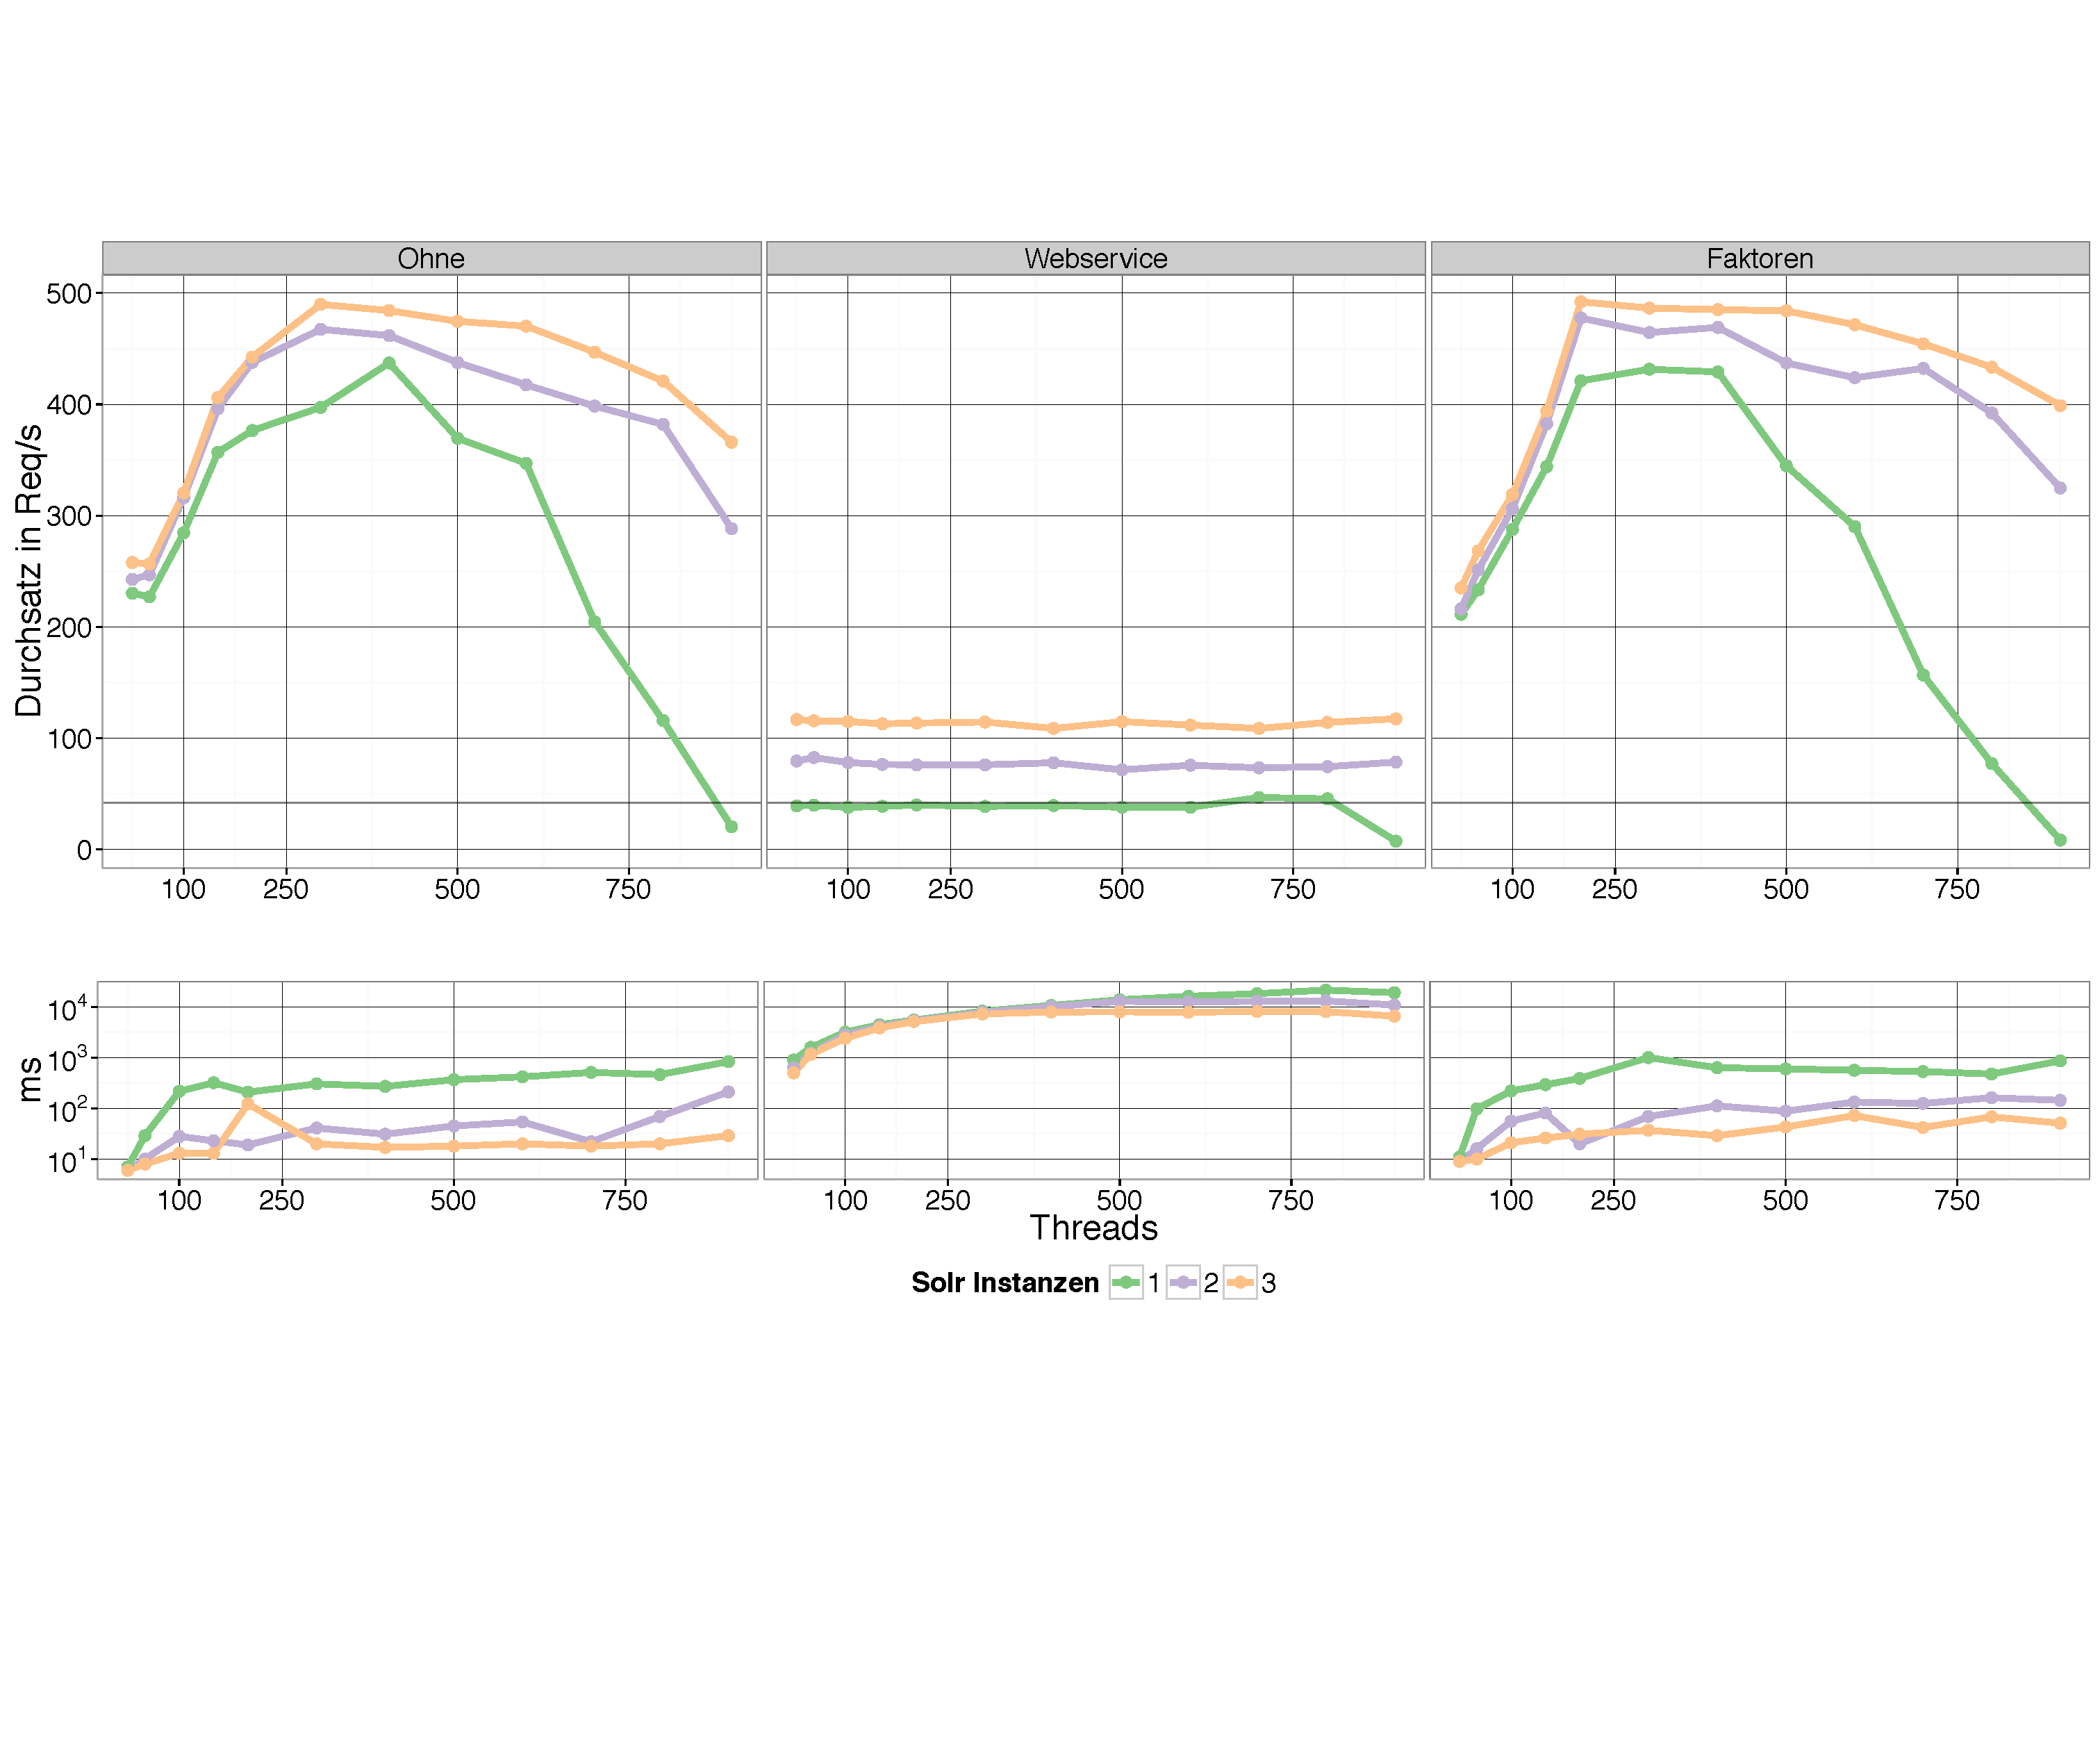
\includegraphics[width=\textwidth]{Abbildungen/personalisierung.pdf}
    \caption[Leistung d. personalisierten Suche]{Leistungsvergleich der Solr-Instanzen mit verschiedenen Personalisierungslösungen für verschiedene Parallelisierungs- und Skalierungsstufen}
    \label{fig:chart_solr}
\end{figure}

\paragraph{Integrierte Personalisierung}

\subsubsection{Qualität}

\begin{SCtable}
  \centering
  \begin{tabular}{ l | r  r  }
  %\cline{2}
  Alogrithmus & RMSE \\ \hline
  Item-Item (Cosine) & 0.9730 \\ 
  Item-Item (Euclid) & 1.1131 \\   
  Item-Item (Jaccard) & 0.9616 \\
  Item-Item (Pearson) & 0.9723 \\ \hline
  NSVD2 & 0.9840  \\
  SVD &	0.9062 \\ \hline
  Zufall &	1.7358
  \end{tabular}
  \caption{\footnotesize Evaluationsergebnisse der verschiedenen vorgestellten Recommender-Algorithmen mit Apache Mahout  (vgl. Abschnitt \ref{sec:filtermethods}). { \scriptsize (eigene Abbildung)}}
  \label{tab:rmse-eval}
\end{SCtable}

\begin{itemize}
\item Qualität Personalisierung 1 - Metrik RMSE (Euclid, Pearson, Kosinus, Jaccard)
\item Qualität Personalisierung 1 - Nachbarschaftsgröße (20,30,40,50)
\item Qualität Personalisierung 2 - Metrik RMSE
\end{itemize}

\subsection{Diskussion}

Cremonesi10 - Abwägung RSME / Pression / Recall Messung bei Top-N Recommendern \\
Howe08 - Abwägung der versch. Distanzmaße zwischen Datensätzen

Skalierbarkeit evt. mit weiterem Datensatz ``testen'': \\
\url{http://aws.amazon.com/datasets/6468931156960467} -> (Subset: \url{http://labrosa.ee.columbia.edu/millionsong/tasteprofile}) \\

Signifikanz: \url{http://www.mitp.de/imperia/md/content/vmi/1634/1634_kapitel_20.pdf} \\
Joachim05 -> Wilcoxon test